% !TeX root = ../thuthesis-example.tex

\chapter{实现初步的出租车调度系统的跨链交易}

\section{实验说明}

在之前第四章的实验中,我们做了现有的基于区域搜索的树状区块链中的一条虚拟父链之下的多个子链内部的并行调度操作,验证了树状区块链在每条单链中运行出租车调度系统的可行性,并且测试了树状多链区块链的性能。但是,在之前的测试中,相互匹配的乘客与车辆账户均处于树状区块链的同一条子链当中,所有的搜索,导航,以及付款交易的操作均是在一条子链中完成;事实上这并不符合实际应用场景,因此,本章的内容主要就是围绕如何实现出租车调度系统的跨链交易来展开。在本章中,笔者给出了跨链交易的较为完整的逻辑架构,但是由于时间有限,笔者重点完成了跨链转账的实现,将转账过程通过合约的事件交互实现,并将整个过程封装进一个函数,提供接口,使其整体形成一个原子操作,同时还实现了资产回流的操作,验证乘客是否确认上车,若成功上车则继续订单,若没成功上车,则触发资产回流;此外,笔者还修改了测试脚本的逻辑架构,使其更符合实际的应用情景,有关跨链搜索以及账户跨链后的资产转移部分目前完成的不够完善,仅服务于测试实验,后续若有时间,笔者也愿意接着进行后续的跨链交易的研究。

\section{实验逻辑介绍}

基于现有的出租车调度系统,为了实现不同子链之间的跨链交易,我们主要需要修改的部分主要有四点:

\begin{enumerate}
    \item 整体测试代码的逻辑架构
    \item 车辆选择的过程
    \item 乘客账户向车辆账户支付订单的过程(即跨链转账)
    \item 乘客账户及车辆账户随位置改变而进行账户资产转移的过程
\end{enumerate}

如图\ref{fig:出租车调度系统的跨链交易运行流程图}所示,相较于第四章中较为简单的调度过程,跨链的出租车调度系统的逻辑过程更加复杂。

\begin{figure}
	\centering
	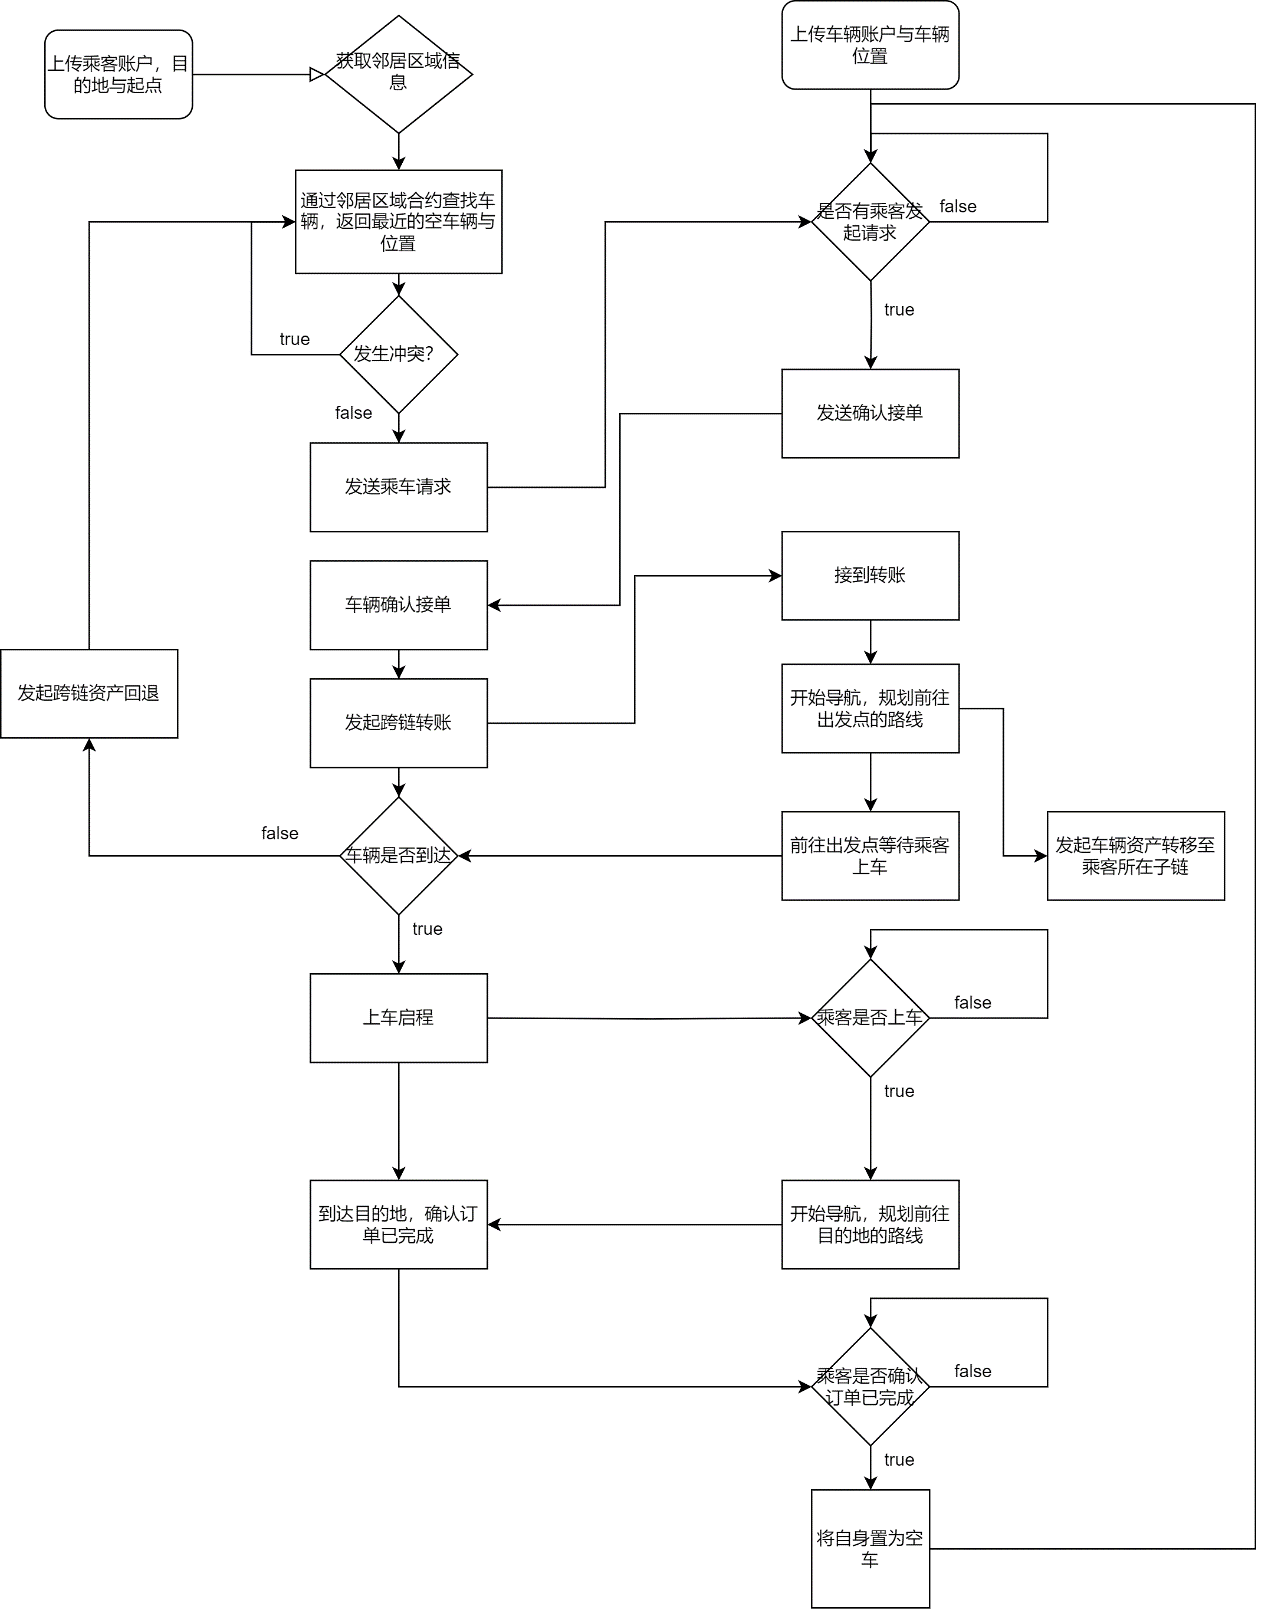
\includegraphics[width=\textwidth]{figures/出租车调度系统的跨链交易运行流程图.png}
	\caption{出租车调度系统的跨链交易运行流程图}
	\label{fig:出租车调度系统的跨链交易运行流程图}
\end{figure}

对于乘客端而言其操作流程大致为:

\begin{enumerate}
    \item 上传起点与目的地
    \item 获取邻居信息,初始设定搜索半径r,判断初始起点位置周围的半径的r圆是否进入了别的邻居区域,若不进入,则仍是简单的单子链内的操作;若进入,则通过父链获取邻居的合约地址,按顺序调用合约的getVehicle函数,汇总结果,得到最近的车辆及其账户,判断此交易是否需要跨链(若不跨链则仍是单子链内操作,本章内容主要考虑需要跨链的情况下的处理,因此,接下来的描述中默认匹配到的车辆需要跨链操作)。
    \item 选择车辆等待确认(这一步触发异步机制,同时只有同一个乘客可以选择一个车辆),在车辆确认接单后,发起跨链的转账。
    \item 跨链转账完成后,还需要考虑交易终止的资产回退问题,若车辆未能到达,乘客未能上车,则会触发跨链的资产回退
    \item 乘客上车启程之后,等待到达目的地时向车辆发送一个确认订单结束。
\end{enumerate}

对于车辆端而言其操作流程大致为:

\begin{enumerate}
    \item 上传起点与目的地
    \item 有乘客请求之后,向乘客发送确认接单
    \item 在跨链转账完成后,开始导航并规划前往乘客出发点的路线
    \item 注意车辆在运动到乘客所在子链区域之后,需要触发车辆的跨链资产转移
    \item 等待乘客上车后,开始导航并规划前往乘客目的地的路线
    \item 收到乘客的订单确认信息后,结束订单,将车辆状态置为空车
\end{enumerate}


\section{完成跨地区之间的车辆搜索}

\subsection{实验思路及实际修改}

本小节主要实现上述过程中的跨区域的车辆搜索问题,在本次实验中,实验规模仅仅涉及3个相邻区块,因此初始在终端中直接记录了相关的合约地址进行调用。

具体实现大致为:获取邻居信息,初始设定搜索半径r,判断初始起点位置周围的半径的r圆是否进入了别的邻居区域(此处默认搜索范围进入了相邻区块中),通过邻居的合约地址,按顺序调用合约的getVehicle函数,汇总结果,得到最近的车辆及其账户。选择车辆等待确认(这一步触发异步机制,同时只有同一个乘客可以选择一个车辆),若车辆已被占用,则等待一段时间后再次重复上述步骤。

其中,对于智能合约的修改是修改了原有的getVehicle。原本的单链程序中搜索车辆的过程是,首先获取本链中的所有车辆账户,并以此根据geohash编码计算曼哈顿距离筛选出离乘客最近的车辆,这在实际应用中是不合法的行为,修改了getVehicle,使得整个搜索过程都封装在了合约中进行,乘客能做的便是调用该合约函数,并得到返回的车辆账户的账户以及位置信息。

整体实验仓库基于第4章的实验进行,实验在真实世界地图中 Geohash 编码前缀为wx4e的区域下进行。树状区块链部分的实验在该区域下的细分区域 wx4en、wx4ep、wx4eq和wx4er区域下进行。

由于本节主要测试跨链搜索的实现的正确性,故主要选取了wx4en、wx4ep、wx4eq三条子链,其中在wx4en中初始部署乘客账户,在wx4ep、wx4eq中部署车辆账户,运行修改后的测试脚本,测试跨链搜索的实现是否正确。

在本小节的实验中,笔者仅仅测试了跨链的车辆搜索的过程,之后的跨链转账以及车辆资产转移并未修改。代码仓库详见:

\subsection{实验测试}

如图在wx4en区域设立了两个乘客,并不设置车辆账户,分别在wx4ep、wx4eq中各设立一个车辆账户,基本测试数据还是用第4章中的点位数据

如表6-2中所示之点位,作为本章测试的测试数据集。

\begin{table}[htbp]
    \linespread{1.5}
    \zihao{5}
    \centering
    \caption{测试数据位点}\label{测试数据位点}
    \begin{tabular}{c|c|c|c} \toprule
        区域Geohash前缀 & 乘客起点        & 乘客终点        & 司机初始位置      \\\hline
        wx4en       & wx4enscgue5 & wx4enrq9mm9 & wx4enrq9mm9 \\
        wx4ep       & wx4epb8scg1 & wx4ep8e5gw0 & wx4ep8e5gw0 \\
        wx4eq       & wx4eq7rgmxk & wx4eqt6u0vu & wx4eqt6u0vu \\
        wx4er       & wx4erd4xkyz & wx4erw9rmze & wx4erw9rmze \\
        \bottomrule
    \end{tabular}
\end{table}

实验具体流程如仓库所示:

\begin{enumerate}
    \item 准备测试用的司乘数据,结果存于仓库中的json格式的文件中。
    \item 按照操作顺序启动三条子链,构建三子链网络,确保初始账号相同,且账号解锁。
    \item 在三子链上分别部署合约,并在乘客端和司机端的测试脚本中更新合约地址。
    \item 上传地图文件。
    \item 依次启动三条子链开始挖矿,同时运行乘客端和司机端的测试脚本,等待测试结束。
    \item 根据输出日志判断,跨链搜索实验是否成功。
\end{enumerate}

\subsection{实验结果}

在搜索过程中,车辆端的实验日志输出如下,具体可详见仓库中的实验截图:

\begin{verbatim}

accountAddr:0xdedee68f2020c0d3f98d2a8c23b6563f7b97e559
车辆正在上传位置
车辆账户加入:0xdedee68f2020c0d3f98d2a8c23b6563f7b97e559
wx4ep8e5gw0第1辆车加入
Myevent:Myevent_vehicleId: 
0xdedee68f2020c0d3f98d2a8c23b6563f7b97e559000000000000
000000000000
Send_Confirm:0xdedee68f2020c0d3f98d2a8c23b6563f7b97e559
Beginevent:Beginevent_vehicleId: 0xdedee68f2020c0d3f98d
2a8c23b6563f7b97e559000000000000000000000000
0xdedee68f2020c0d3f98d2a8c23b6563f7b97e559接到了乘客 
0x12d0e4381ef94a70a49252e35b9a65fadd3872b90000000000000
00000000000 的订单, 乘客位置:  wx4epb8scg1

\end{verbatim}

\begin{enumerate}
    \item 准备测试用的司乘数据,结果存于仓库中的json格式的文件中。
    \item 按照操作顺序启动三条子链,构建三子链网络,确保初始账号相同,且账号解锁。
    \item 在三子链上分别部署合约,并在乘客端和司机端的测试脚本中更新合约地址。
    \item 上传地图文件。
    \item 依次启动三条子链开始挖矿,同时运行乘客端和司机端的测试脚本,等待测试结束。
    \item 根据输出日志判断,跨链搜索实验是否成功。
\end{enumerate}

表明本小节实现的跨链搜索可以正确运行。

\section{实现不同地区之间的交易转账}

\subsection{实验思路及实际修改}

本小节也是本章的重点,主要实现的是如图6-1中跨链转账的部分。在实际应用场景当中,预付款或者提前支付定金是十分必要的,在此前的树状区块链出租车调度系统当中,仅仅支持同一条子链内部的转账操作,且其是在乘客确认订单完成后,才会发起转账支付。虽然在车辆进入到乘客所在的子链区域范围后,通过车辆账户的自身跨链资产转移可以满足乘客与车辆进行交易的条件,但是实际应用场景中,提前支付或者支付定金是对司机权益的一种保障,否则如果乘客中途退单,司机就会有空车返回的风险。本小节的主要实现目标便是希望树状区块链的出租车调度系统也可以满足跨链的提前支付。

本小节内容主要基于第五章《基于树状区块链的跨链转账测试》来做。在第五章中已经介绍过,一个账户在跨区域时需要将账户金额转移至目标区域的子链的这一过程,笔者根据此操作并结合源码,测试并验证出了跨链转账的可行性,笔者将此功能封装进了一个函数,并给出了一个具有较高鲁棒性且便于调用的函数接口,在上述的6.3小节的实验基础上,测试并实验不同地区账户之间的转账操作。

在本小节的实验中,笔者在跨链搜索车辆的基础上测试了之后的跨链转账过程,后续的车辆资产转移部分并未修改,故最终验证结果时,也还是在车辆的原有链中验证车辆账户余额。

\subsection{跨链转账的过程}

如图\ref{fig:出租车调度系统的跨链转账示意图}所示,跨链转账的过程:

\begin{figure}
	\centering
	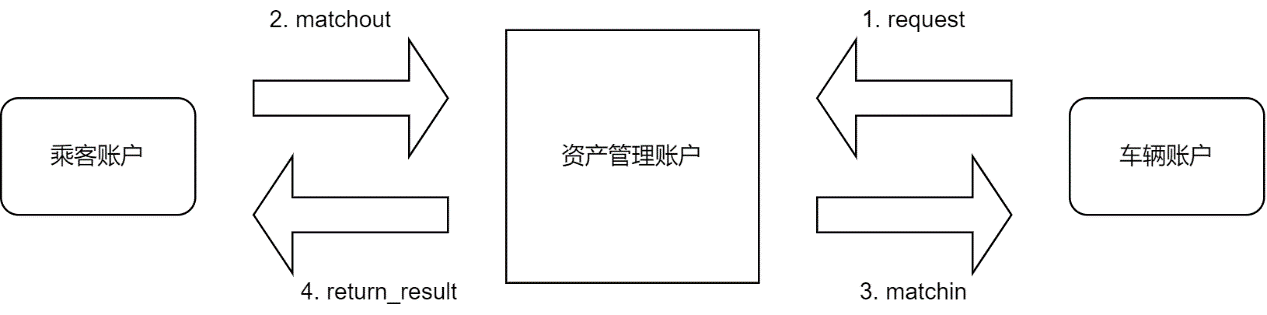
\includegraphics[width=\textwidth]{figures/出租车调度系统的跨链转账示意图.png}
	\caption{出租车调度系统的跨链转账示意图}
	\label{fig:出租车调度系统的跨链转账示意图}
\end{figure}

\begin{enumerate}
    \item 首先是车辆账户需要向分支节点的资产管理账户发送一个request请求,同时,通过合约函数发送交易双方的账户,以及request请求产生的hash值。
    \item 乘客端接收到该事件后,乘客端会向分支节点的资产管理账户发送一个matchout转账请求,同时,乘客端通过合约函数发送交易双方的账户转账金额,以及matchout请求产生的hash值。
    \item 车辆端接收到该事件后,分支节点的资产管理账户会向车辆端发送一个matchin转账请求,同时,通过合约函数发送交易双方的账户转账金额,以及matchin请求产生的hash值。
    \item 乘客端接收到该事件后,表明此时matchout和matchin请求都已成功,分支节点的资产管理账户会向乘客端发送一个return-result请求,记录并验证交易结果。
\end{enumerate}

\subsection{实验测试}

本小节的实验基于第六章第3小节中的实验来做,实验数据选取的是,6.3小节中的实验数据。具体操作流程以及代码修改详见本人的毕设仓库。

实验具体流程如仓库所示,大致流程如下:

\begin{enumerate}
    \item 准备测试用的司乘数据,结果存于仓库中的json格式的文件中。
    \item 按照操作顺序启动三条子链,构建三子链网络,确保初始账号相同,且账号解锁。
    \item 在三子链上分别部署合约,并在乘客端和司机端的测试脚本中更新合约地址。
    \item 上传地图文件
    \item 依次启动三条子链开始挖矿,同时运行乘客端和司机端的测试脚本,等待测试结束。
    \item 重启区块链,重做一个不含转账的对照试验,依次启动三条子链开始挖矿,同时运行乘客端和司机端的不转账测试脚本,等待测试结束。
    \item 重启区块链,重做一个转账到目标链的非车辆也非乘客的账户的实验,依次启动三条子链开始挖矿,同时运行乘客端和司机端的不转账测试脚本,等待测试结束。
    \item 根据输出日志验证跨链转账交易流程的正确性。
    \item 在命令行查验车辆账户余额,对比车辆账户金额验证跨链转账交易是否成功。
\end{enumerate}

\subsection{实验结果}

在实验过程中,乘客端的实验日志输出如下,具体可详见仓库中的实验截图(包含日志输出截图以及账户余额截图)

\begin{verbatim}

开始支付订单
vel 0xdedee68f2020c0d3f98d2a8c23b6563f7b97e559
res: 0xa683e5d4982e63a9b4babbab21aad1090c673806ad98ba98
dfab582bedd368e3
hash_request: 0x307861363833653564343938326536336139623
4626162626162323161616431303930633637333830366164393862
61393864666162353832626564643336386533
get_outchain_info--outchain_balance: 100000000000000
Result: 0x7e61314b0e7b5ae7c229cebfc71657bebf9cd48eda
ae0702933bd9471af19bd7
乘客支付了订单
send_inchain--Result: 0xc27f230d538a429049565caf52b63d3
f2bbc3605558d4d630ec0cad0c95c3dca
send_inchain--hash_in: 0x307863323766323330643533386134
3239303439353635636166353262363364336632626263333630353
53538643464363330656330636164306339356333646361
send_inchain--balance: 100000000000000
send_result--Tx_result: 0x78be78c00f0aae68e2e93fdc1676b
bc78d0eacf82b994ab1b891dfd1c6de9b1c
乘客确认交易结束

\end{verbatim}

表明本小节实现的跨链转账交易可以正确运行。经过在命令行查看车辆账户余额,可以看到:

如表6-1中所示,分配实验账户:

\begin{table}[H]
    \linespread{1.5}
    \zihao{5}
    \centering
    \caption{实验账户公钥}\label{实验账户公钥}
    \begin{tabular}{cc} \toprule
        乘客车辆账户                  & 公钥                         \\ \hline
        Wxtep链中的车辆账户acc1 & 0xdedee68f2020c0d3f98d2a8c23b6563f7b97e559            \\
        Wxteq链中的车辆账户acc2   & 0xad8a321e2e8f8f51245f47b8f412979d5740e625            \\
        Wxten链中的乘客账户acc3   & 0x12d0e4381ef94a70a49252e35b9a65fadd3872b9 
        \\
        Wxten链中的乘客账户acc4   & 0x456c4df0610c7611ae8bcaed32dd1d94e88ceca4
        \\\bottomrule
    \end{tabular}
\end{table}

账户初始金额:50000000000000000000
如表6-2所示:

\begin{table}[H]
    \linespread{1.5}
    \zihao{5}
    \centering
    \caption{实验结果}\label{实验结果}
    \begin{tabular}{ccc} \toprule
        账户类别                & 账户                 & 转账的试验后金额           \\ \hline
        Wxtep链中的车辆账户 & acc1   & 50000892848000000000                \\
        Wxteq链中的车辆账户 & acc2   & 50000892848000000000                \\
        Wxten链中的乘客账户 & acc3   & 49998851463000000000 
        \\
        Wxten链中的乘客账户 & acc4   & 49998866463000000000
        \\\bottomrule
    \end{tabular}
\end{table}

结果显示,车辆账户收到转账,验证了本节实现的跨链转账的正确性。
注意到本区块链中两个账户使用相同的合约函数发送相同的请求,send中设定的gas值也一样,但最终消耗的gas值不一样,笔者推测这可能是因为第一次调用该函数会触发合约代码的初始化,需要加载更多的资源和执行更多的操作,因此会消耗更多的gas。而后续的调用由于已经完成了初始化,所以消耗的gas会稳定在一个较小的范围内。

\section{将上述操作封装进智能合约}

\subsection{实验思路及实际修改}

将上述测试脚本的运行逻辑进行改进,使得整个过程都是基于合约中的事件来触发,修改了原有的traffic合约,并新实现了一个transfer合约用于跨链转账的过程中进行通信交互,使得整体过程更趋于实际的应用过程。并且将该过程由合约封装后,在实际的高负载应用中维护跨链转账交易的原子性;同时,实际转账操作也对用户隐藏,对外仅提供将转账的操作由合约函数接口来执行此功能。

% \subsection{算法}

% 算法环境可以使用 \pkg{algorithms} 或者 \pkg{algorithm2e} 宏包。

% \renewcommand{\algorithmicrequire}{\textbf{输入:}\unskip}
% \renewcommand{\algorithmicensure}{\textbf{输出:}\unskip}

% \begin{algorithm}
%   \caption{Calculate $y = x^n$}
%   \label{alg1}
%   \small
%   \begin{algorithmic}
%     \REQUIRE $n \geq 0$
%     \ENSURE $y = x^n$

%     \STATE $y \leftarrow 1$
%     \STATE $X \leftarrow x$
%     \STATE $N \leftarrow n$

%     \WHILE{$N \neq 0$}
%       \IF{$N$ is even}
%         \STATE $X \leftarrow X \times X$
%         \STATE $N \leftarrow N / 2$
%       \ELSE[$N$ is odd]
%         \STATE $y \leftarrow y \times X$
%         \STATE $N \leftarrow N - 1$
%       \ENDIF
%     \ENDWHILE
%   \end{algorithmic}
% \end{algorithm}

\subsection{实验测试}

本小节的实验基于第六章第4小节中的实验来做,本小节实验需要验证跨链转账操作的原子性,故引入单链中的冲突事件,初始设定10个账户参与测试(4个车辆账户,wx4ep区域中2个,wx4eq区域中2个;6个乘客账户,均位于wx4en区域中),实验的位点数据选取的仍是,6.4小节中的实验数据。具体操作流程以及代码修改详见本人的毕设仓库。

\subsection{实验结果}

在实验过程中,实验日志输出如下,具体可详见仓库中的实验截图(包含日志输出截图以及账户余额截图):

\begin{verbatim}
    IN_transf1
    IN_Event1
    send_inchain--Result: 0xc27f230d538a429049565caf52b
    63d3f2bbc3605558d4d630ec0cad0c95c3dca
    send_inchain--hash_in: 0x30786332376632333064353338
    613432393034393536356361663532623633643366326262633
    336303535353864346436333065633063616430633935633364
    6361
    send_inchain--balance: 100000000000000
    send_result--Tx_result: 0x78be78c00f0aae68e2e93fdc1
    676bbc78d0eacf82b994ab1b891dfd1c6de9b1c
    OUT_Event2
    send_result--Tx_result: end
    IN_Event3
    RE_Event4
\end{verbatim}

日志中输出了合约函数的调用信息,表明本小节实现的跨链转账交易的合约封装可以正确运行。经过在命令行查看车辆账户余额,可以看到:

如表6-1中所示,分配实验账户:

\begin{table}[H]
    \linespread{1.5}
    \zihao{5}
    \centering
    \caption{实验位点}\label{实验位点}
    \begin{tabular}{cc} \toprule
        乘客车辆账户                  & 账户地址                                           \\ \hline
Wxtep链中的车辆账户acc1 & 0x7a68b86008b0cfc3ae0e8068360271cbb999c97d
        \\
Wxtep链中的车辆账户acc2   & 0xd5f5ef5ff4c6323c62bdc5ab2061f440aefc511b    
        \\
Wxteq链中的车辆账户acc3   & 0xd402c7301a68c4c65529ab0c597bb8b13e27f607
        \\
Wxteq链中的车辆账户acc4   & 0x42389309e69a2b32b98f04bc8255ad971797f757
        \\
Wxten链中的乘客账户acc5  & 0xdedee68f2020c0d3f98d2a8c23b6563f7b97e559
        \\
Wxten链中的乘客账户acc6   & 0xc0a3917e5679c0ef9033c41cbe294a212abe55df             \\
Wxten链中的乘客账户acc7   & 0x55577fd620a0b8379846fcb1499e4bdc22538843
        \\
Wxten链中的乘客账户acc8   & 0xad8a321e2e8f8f51245f47b8f412979d5740e625
        \\
Wxten链中的乘客账户acc9  & 0x91153bad44dcc46187c481d8d36a53e58522d0c4
        \\
Wxten链中的乘客账户acc10   & 0xe64e81bc77ee05caaa6b1476de75193607e84d87                             
        \\\bottomrule
    \end{tabular}
\end{table}

账户初始金额:50000000000000000000
如表6-2所示:

\begin{table}[H]
    \linespread{1.5}
    \zihao{5}
    \centering
    \caption{Wxtep链中的车辆账户}\label{Wxtep链中的车辆账户}
    \begin{tabular}{*{5}{>{\centering\arraybackslash}p{6cm}}} \toprule
        账户                & 转账的试验后金额           \\ \hline
        acc1   & 50000907848000000000               \\
        acc2   & 50001892848000000000              \\
        \bottomrule
    \end{tabular}
\end{table}

\begin{table}
  \centering
  \caption{Wxteq链中的车辆账户}
  \begin{tabular}{*{5}{>{\centering\arraybackslash}p{6cm}}}
    \toprule
    账户                & 转账的试验后金额        \\
    \midrule
    acc3   & 50000907848000000000               \\
    acc4   & 50001892848000000000               \\
    \bottomrule
  \end{tabular}
  \label{tab:Wxteq链中的车辆账户}
\end{table}

\begin{table}[H]
    \linespread{1.5}
    \zihao{5}
    \centering
    \caption{Wxten链中的乘客账户}\label{Wxten链中的乘客账户}
    \begin{tabular}{*{5}{>{\centering\arraybackslash}p{6cm}}} \toprule
        账户                & 转账的试验后金额           \\ \hline
        acc5   & 49998851463000000000               \\
        acc6   & 49998866463000000000               \\
        acc7   & 49998866463000000000               \\
        acc8   & 49998866463000000000               \\
        acc9   & 49998866463000000000               \\
        acc10   & 49998866463000000000              \\
        \bottomrule
    \end{tabular}
\end{table}

如表6-3所示,可以看出含转账的实验中金额是明显多于未转账的,转账实验验证成功。同时,转账事件之间并无冲突,验证了跨链转账操作的原子性实现的正确性。

\section{实验不足性说明}

\subsection{搜索方面的简化}

在搜索车辆时,需要获取邻居子链的合约的地址信息,这部分操作需要与父链相结合来完成,目前并未完整的实现与父链进行交互的这一搜索过程。而是为了简化验证跨链搜索的正确性直接在终端部署了邻居子链的合约地址。

\subsection{车辆运行的简化}

在实际的应用程序中,应该要能够实时展示乘客与车辆的位置信息,并且要及时将位置信息上传到区块链当中,此部分目前并未与前端相结合实现,由于本章重点验证的跨链交易的实现,故在测试脚本代码中省略了车辆调度过程中时时上传地理位置信息的操作。

\subsection{资产转移的省略}

在车辆跨链进入乘客所在的子链时,需要触发车辆账户的资产转移,本事件并未在本章节中体现,不过,跨链资产转移的实现以及相关测试第五章中均已完成,故后续在本章节中添加资产转移的事件的话也是一件较为轻松的工作,笔者在此简单叙述一下实现了逻辑过程,在车辆实时上传地理位置信息的操作前添加对于位置信息的判断,若超出了当前所处链的范围,则需触发跨链的资产转移。

\section{本章小结}

本章的内容主要就是围绕如何实现出租车调度系统的跨链交易来展开。在本章中,笔者给出了跨链交易的较为完整的逻辑架构,同时完成了其中的跨链转账的实现,将转账过程通过合约的事件交互实现,并将整个过程封装进一个函数,提供接口,使其整体形成一个原子操作,同时还实现了资产回流的操作,验证乘客是否确认上车,若成功上车则继续订单,若没成功上车,则触发资产回流;此外,笔者还修改了测试脚本的逻辑架构,使其更符合实际的应用情景。

目前实验的不足在于有关跨链搜索以及账户跨链后的资产转移部分目前完成的尚不够完善,仅服务于测试实验,笔者给出了其实际应用情形的逻辑架构,便于后续研究者的研究与实现,后续若有时间,笔者也愿意接着进行后续的跨链交易的研究。
